\documentclass[11pt]{article}
\usepackage{geometry}
\usepackage{lipsum}
\usepackage{multicol}
\usepackage{enumitem}
\usepackage{fancyhdr}
\usepackage[english]{babel}
\usepackage[sc]{mathpazo}                   
\usepackage{graphics}
\usepackage{graphicx}

\usepackage{algorithm}
\usepackage{algorithmic}
\renewcommand{\algorithmicrequire}{\textbf{Input:}}
\renewcommand{\algorithmicensure}{\textbf{Output:}}

\usepackage[%  
    colorlinks=true,
    pdfborder={0 0 0},
    linkcolor=red
]{hyperref}

\setlist[itemize]{noitemsep, topsep=0pt}
\setlist[enumerate]{noitemsep, topsep=0pt}

\pagestyle{fancy}
\renewcommand{\headrulewidth}{0pt}
\newcommand{\bb}[1]{\textbf{#1}}


\graphicspath{ {./imgs/} }

\fancyhead[L]{CSCI 545: Introduction to Robotics}
\fancyhead[R]{Fall 2019}

\title{Lecture 17: \it{Motion Planning I}}
\author{Scribe:  \it{Duong Le, Keyu Han, Baiyu Huang, Seunghee Yoon, Guifan Weng}}
\date{}


\begin{document}
\maketitle
\thispagestyle{fancy}
\section{Complete Motion Planning}

\subsection{Element of Motion plan}
Motion plan generally takes the elements followings into the considerations. 
\begin{itemize}
\item \textbf{Plans} \{Discrete, Continous, Hibrid\} \\
This category indicates whether a certain plan covers a discrete number space or a continuous one. For instance, grasping an object in a continuous space while make a decision among discrete classes would belong to Hybrid plans.
\item \textbf{Environment} \{Immovable, Movable, Moving\}\\
This is the environment where an agent moves. The example of Immovable environment can be fixed obstacles such as walls while movable ones are Movable objects like apples, chairs. Moving objects are literally the non-fixed object on the fields such as animals, humans.
\item \textbf{Interaction} \{None-Contact, Contact\}\\
An agent interacts with the environment, which should be considered during planning. None-Contact interaction is the interaction where the agent tries to avoid a collision while Contact embraces situations such as grasping, pushing, or pulling an object.
\item \textbf{Uncertainty} \{Node, Known, Bounded, Unknown\}\\
‘Node’ refers to given configuration spaces q while ‘Known’ does to the position according to the configurations, which is p(q). ‘Bounded’ refers to restrict conditions that bound our configurations (ex, q must belong to Q). ‘Unknown’ indicates unknown configuration that we need to figure out. Usually, the unknown configuration is a semi solution or solution itself of entire planning problems. 
\item \textbf{Robot Motion} \{Kinematic, Dynamics\}\\
Kinematic setting describes a robot motion with configuration q while Dynamics does with configuration and its derivative q’ that is, the velocity of q.
\end{itemize}
\subsection{Problem Formulation(piano mover's problem )}
Figure \ref{fig:pmp} describes the elements of Piano mover’s problems with which we will usually deal in motion panning. The criteria settings of the problems are the followings:
\begin{itemize}
\item A world with $R^2$ or $R^3$ spaces.  
\item Obstacles occupies a space Cobs ($Q_{obs}$) in the world
\item A robot and its configuration space $C(Q)$ 
\item Where $Q_{free} = Q\setminus Q_{obs}$, $qs$ is in $Q_{free}$ at the initial configurations; and so is $qg$. $Q_{free}$ is the configuration spaces that are not occupied with obstacles. 
\end{itemize}
\begin{figure}[h]
  \centering
  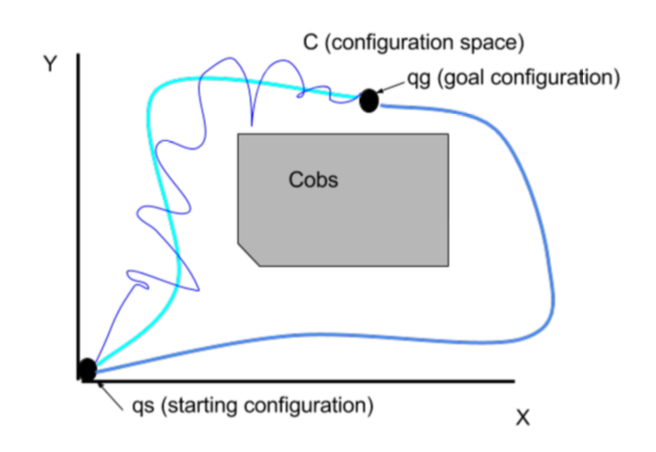
\includegraphics[width=12cm]{piano_movers_problem.png}
  \label{fig:pmp}
  \caption{piano movers problem}
\end{figure}
For short, our goal as to that problem is to come up with a function that executes the mapping $T:[0, 1] \rightarrow Q_{free}$ where $qs = T(0)$ and $qg = T(1)$. In other word, this is finding a path specifying configurations corresponding to each time steps between 0 and 1. 
\subsection{Cell Decompose}
Considering the contents above, it is obvious that how to represent and know free space is a crucial issue to solve piano mover’s problems. Cell Decompose is a category of a method to represent the free space where the free spaces are the set of ‘cells’ into which the free spaces are separated. Trapezoidal decomposition algorithm is one of them. Each node corresponds to a cell and an edge connects nodes of adjacent cells forming graphs. After the cell decomposition, path planning with a cell decomposition is usually done in two steps: first, the planner determines the cells that contain the start and goal, respectively, and then the planner searches for a path within the adjacency graph. Note that the adjacency graph could serve as a roadmap of the free space as well. If there is one ore more path that connects start and goal, that means there is a path among the road map; thus, this solution is roadmap based method as well where it is guaranteed to derive a solution from a roadmap or at the very least know there is no valid route. Yet, this method can only be applied to simple spaces.
\subsubsection{Algorithm}
\begin{figure}[h]
  \centering
  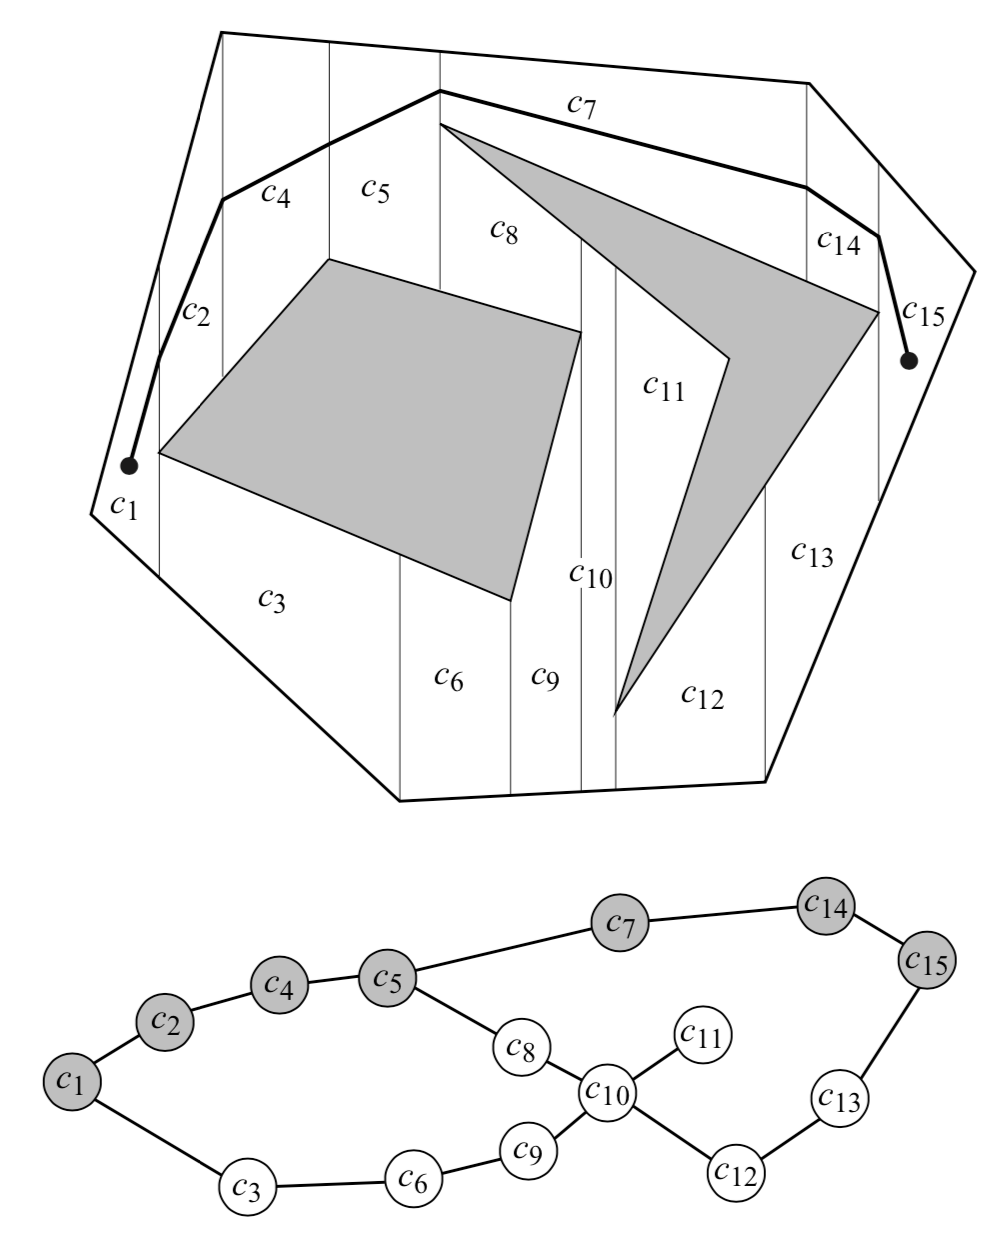
\includegraphics[width=10cm]{cell_decompose.png}
  \caption{cell decompose}
  \label{fig:cell_decompose}
\end{figure}
Fig \ref{fig:cell_decompose} The resulting paths in the adjacency graph and free space. The straight lines up and down are called ‘boundary’ while the separated areas (cells) are ‘trapajoid’.

We assume all the vertices and their Euclidean positions are known. Then for each vertex, do the following steps.
\begin{itemize}
  \item Draw line heading to upper and bottom from the vertex until it meets an intersection.
  \item Sample a point in every trapezoid and its boundary; these points will be saved as nodes of a graph. Note that every boundary line must exclude an intersection.
\end{itemize}
After doing that, find the trapezoid where our start and goal belongs to; and connect all the nodes forming a graph. Then, one can easily find a path by using the graph search algorithms such as DFS, or BFS.

\subsection{Visibility Graph}

The defining characteristics of a visibility map are that its nodes share an edge if they are within line of sight of each other, and that all points in the robot's free space are within line of sight of at least one node on the visibility map. This second statement implies that visibility maps, by definition, possess the properties of accessibility and departability. Connectivity must then be explicitly proved for each map for the structure to be a roadmap. In this section, we consider the simplest visibility map, called the visibility graph

\subsubsection{Visibility Graph Definition}


The standard visibility graph is defined in a two-dimensional polygonal configuration space (figure 2.1). The nodes $v_i$ of the visibility graph include the start location, the goal location, and all the vertices of the configuration space obstacles. The graph edges $e_ij$ are straight-line segments that connect two line-of-sight nodes $v_i$ and $v_j$, i.e.,
$$e_ij \ne \emptyset \Longleftrightarrow sv_i + (1-s)v_i \in cl(Q_{free})   \forall s \in [0,1] $$
\begin{figure}[h]
\centering
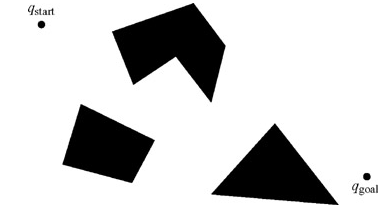
\includegraphics[width=9cm]{imgs/Polygonal_configuration_space.png}
\caption{Polygonal configuration space with a start and goal}
\end{figure}

Note that we are embedding the nodes and edges in the free space and that edges of the polygonal obstacles also serve as edges in the visibility graph.

By definition, the visibility graph has the properties of accessibility and departability. We leave it to the reader as an exercise to prove the visibility graph is connected in a connected component of free space. Using the standard two-norm (Euclidean distance), the visibility graph can be searched for the shortest path . The visibility graph can be defined for a three dimensional configuration space populated with polyhedral obstacles, but it does not necessarily contain the shortest paths in such a space.\\

\begin{figure}[h]
  \centering
  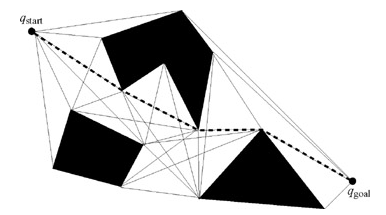
\includegraphics[width=9cm]{imgs/shortest_path.png}
  \caption{The thin solid lines delineate the edges of the visibility graph for the three obstacles represented as filled polygons. The thick dotted line represents the shortest path between the start and goal}
\end{figure}

Unfortunately, the visibility graph has many needless edges. The use of supporting and separating lines can reduce the number of edges. A supporting line is tangent to two obstacles such that both obstacles lie on the same side of the line. For nonsmooth obstacles, such as polygons, a supporting line $l$ can be tangent at a vertex $v_i$ if $\beta_\epsilon(v_i) \bigcap l \bigcap QO_i = v_i $. A separating line is tangent to two obstacles such that the obstacles lie on opposite sides of the line.\\

\begin{figure}[h]
  \centering
  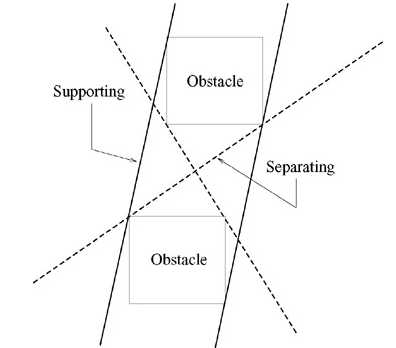
\includegraphics{imgs/Supporting_separating_line_segments.png}
  \caption{Supporting and separating line segments. Note that for polygonal obstacles, we use a nonsmooth notion of tangency}
\end{figure}

The reduced visibility graph is soley constructed from supporting and separating lines. In other words, all edges of the original visibility graph that do not lie on a supporting or separating line are removed. \\

\begin{figure}[h]
  \centering
  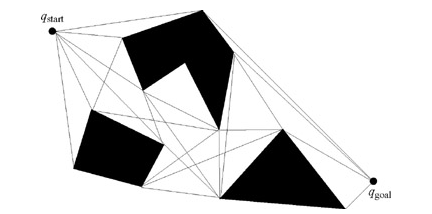
\includegraphics[width=9cm]{imgs/R_V_G.png}
  \caption{Reduced visibility graph}
\end{figure}

\subsubsection{Visibility Graph Construction}
\begin{figure}[h]
  \centering
  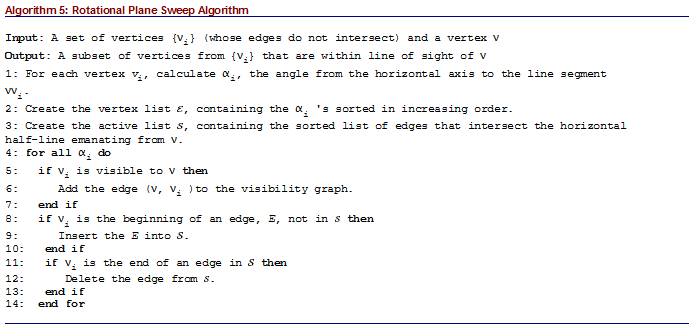
\includegraphics{imgs/Algorithm_5.png}
  \caption{Rotational Plane Sweep Algorithm }
  \label{fig:Algorithm_5}
\end{figure}

Let $V={v_1,...,v_n}$ be the set of vertices of the polygons in the configuration space as well as the start and goal configurations. To construct the visibility graph, for each be the set of vertices of the polygons in the configuration space as well as the start and goal configurations. To construct the visibility graph, for each $v \in V$ we must determine which other vertices are visible to $v$.The most obvious wayto make this determination is to test all line segments $vv_i,v \ne v_i$to see if they intersect an edge of any polygon. For a particular $vv_i$, there are $O(n)$ intersections to check because there are $O(n)$edges from the obstacles. Now, there are $O(n)$ potential segments emanating from $v$,so for a particular $v$, there are $O(n_2)$ tests to determine which vertices are indeed visible from $v$, This must be done for all $v \in V$ and thus the construction of the visibility graph would have complexity $O(n_3)$ \\
There is a more efficient way to compute the set of vertices that are visible from $v$. Imagine a rotating beam of light emanating from a lighthouse beacon. At any moment, the beam illuminates the object that is closest to the lighthouse. Furthermore, as the beam rotates, the obstacle that is illuminated changes only at a finite number of orientations of the beam. If the obstacles in the space are polygons, these orientations occur when the beam is incident on a vertex of some polygon. This insight motivates a class of algorithms known in the computational geometry literature as plane sweep algorithms.\\
A plane sweep algorithm solves a problem by sweeping a line, called the sweep line, across the plane, pausing at each of the vertices of the obstacles. At each vertex, the algorithm updates a partial solution to the problem. Plane sweep algorithms are used to efficiently compute the intersections of a set of line segments in the plane, to compute intersections of polygons, and to solve many other computational geometry problems.\\
For the problem of computing the set of vertices visible from$v$, we will let the sweep line, $l$, be a half-line emanating from $v$,and we will use a rotational sweep, rotating $l$ from 0 to $2\pi$. The key to this algorithm is to incrementally maintain the set of edges that intersect $l$ , sorted in order of increasing distance from $v$. If a vertex $v_i$ is visible to $v$, then it should be added to the visibility graph.It is straightforward to determine if $v_i$ is visible to $v$ (see figure \ref{fig:Algorithm_5}). Let $S$ be the sorted list of edges that intersects the half-line emanating from $v$; the set $S$ is incrementally constructed as the algorithm runs. If the line segment $vv_i$ does not intersect the closest edge in $S$, and if$l$ does not lie between the two edges incident on $v$,(the sweep line does not intersect the interior of the obstacle at $v$), then the $v_i$ is visible to $v$.\\
\newpage
\section{Sampling-based Motion Planning}
Sampling-based motion planning is not complete: not guarantee to find a solution when one exists. However, as the number of samples goes to infinity, there is a strong guarantee that it can find a solution.\\
There are 2 types of sample-based planning algorithms:\\
\begin{multicols*}{2}
\textbf{\underline{Multiple Query Algorithm}}
\begin{itemize}
\item Roadmap is built beforehand. Then it can be used multiple times for different queries.
\item Query is fast since roadmap is already generated.
\item Keeping roadmap all the time is expensive.
\item Can only deal with static environment - has to rebuild the roadmap whenever anything changed in environment.
\end{itemize}
\vfill\null
\columnbreak
\textbf{\underline{Single Query Algorithm}}
\begin{itemize}
\item No roadmap is built beforehand. Find a path from start to goal then finish
\item Query is slower.\\
\item No saved roadmap - better memory \\
\item Can deal with dynamic environment 
\end{itemize}
\end{multicols*}

\subsection{Probabilistic Road Map (PRM)}
Probabilistic Roadmap (PRM) is a multi-query algorithm.\\
There are 2 steps:
\begin{enumerate}
\item Preprocessing state: build roadmap
\item Query state: search roadmap given start and goal
\end{enumerate}

\subsubsection{Roadmap Construction Algorithm}
\begin{algorithm} 
\caption{Roadmap\_Construction\_Algorithm} 
\label{alg:prm_alg} 
  \begin{algorithmic}[1]
  \REQUIRE~~\\
    $n$: number of nodes to put in the roadmap\\
    $k$: number of closest neighbors to examine for each configuration
  \ENSURE~~\\
    A roadmap $G=(V,E)$
    \STATE $V \leftarrow \emptyset$ 
    \STATE $E \leftarrow \emptyset$
    \WHILE {$|V| < n$}
      \REPEAT
    \STATE $q \leftarrow$ a random configuration in $Q$      
      \UNTIL{$q$ is collision-free}
      \STATE $V \leftarrow V \cup \{q\}$
    \ENDWHILE
    
  \FORALL {$q \in V$}
    \STATE $N_q \leftarrow$ the $k$ closest neighbors of $q$ chosen from $V$ according to $dist$
    \FORALL {$q' \in N_q$}
      \IF {$(q,q') \notin E$ {\bf and} $\Delta(q,q') \ne NIL$} 
        \STATE $E \leftarrow E \cup \{(q,q')\}$
      \ENDIF
    \ENDFOR
  \ENDFOR
    \end{algorithmic}
\end{algorithm}

Let $\Delta(q, q')$ be a function that returns either a collision-free path from q to q' or NIL if it cannot find such a path. There are many algorithms can be used for $\Delta$. For example, if we want to check whether there is a straight-line path from q to q, we can use binary search to check for collision.\\
Roadmap construction algorithm shows in Algorithm \ref{alg:prm_alg}:
\begin{itemize}
\item Line (1) and (2): Initialize graph $G=(V,E)$ to be empty.
\item Line (3) to (8) describes sampling process: keep sampling to get $n$ numbers of collision-free samples.
\item Line (9) to the end is process to build roadmap from $n$ samples: for every sample node $q\in V$, create a set $N_q$ of $k$ closest neighbors. Then from every $q' \in N_q$, whenever function $\Delta(q, q')$ succeeds to compute a collision-free path from $q$ to $q'$, the edge $(q,q')$ is added to $E$. Figure \ref{fig:roadmap_example} shows an example of roadmap using $\Delta$ as straight-line planner
\end{itemize}

\begin{figure}[h]
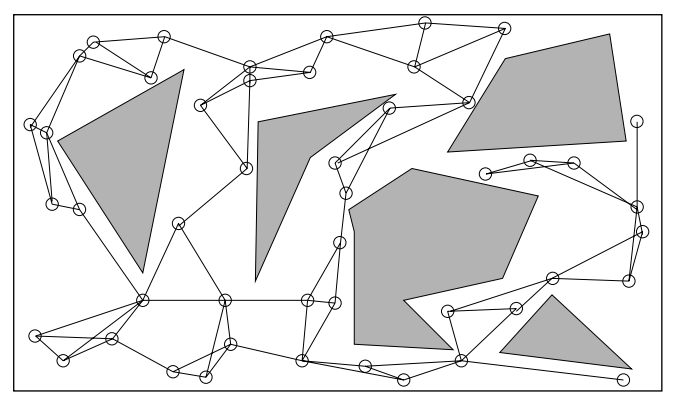
\includegraphics{roadmap}
\centering
\caption{An example of a roadmap }
\label{fig:roadmap_example}
\end{figure}

\subsubsection{Query}
When you have a start point and end point, you connect them to the graph and then using graph searching algorithm to find path from start to end.

\subsubsection{Failure}
If obstacles are very closed to each other, generated roadmap will be disconnected. Possible solution is increasing sampling rate to get more samples. However, probability to sample between the obstacles is very unlikely. For example, in figure \ref{fig:closed_obs}, the chance to sample points in the narrow road between 2 obstacles is very low. If you keep sampling more points, the graph will become so dense and will take a lot of time to find a path between start and end point.\\
\begin{figure}
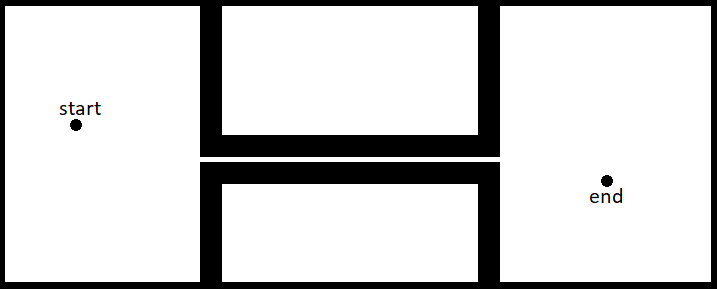
\includegraphics{closed_obs}
\centering
\caption{An example when obstacles are very closed to each other}
\label{fig:closed_obs}
\end{figure}
Solution: sample more points toward edges of the obstacles. We can use binary search to find the closest point to the obstacle that's collision-free, and then sample more points near that point. The process of sampling becomes more expensive, but result graph is less dense and faster to compute path.


\subsection{Visibility PRM}
The roadmap is constructed incrementally by randomly sampling the configuration space and attempting to connect some pairs of collision-free samples by the local method.
The visibility roadmaps are build without any explicit computation of the visibility domains.
\begin{figure}[h]
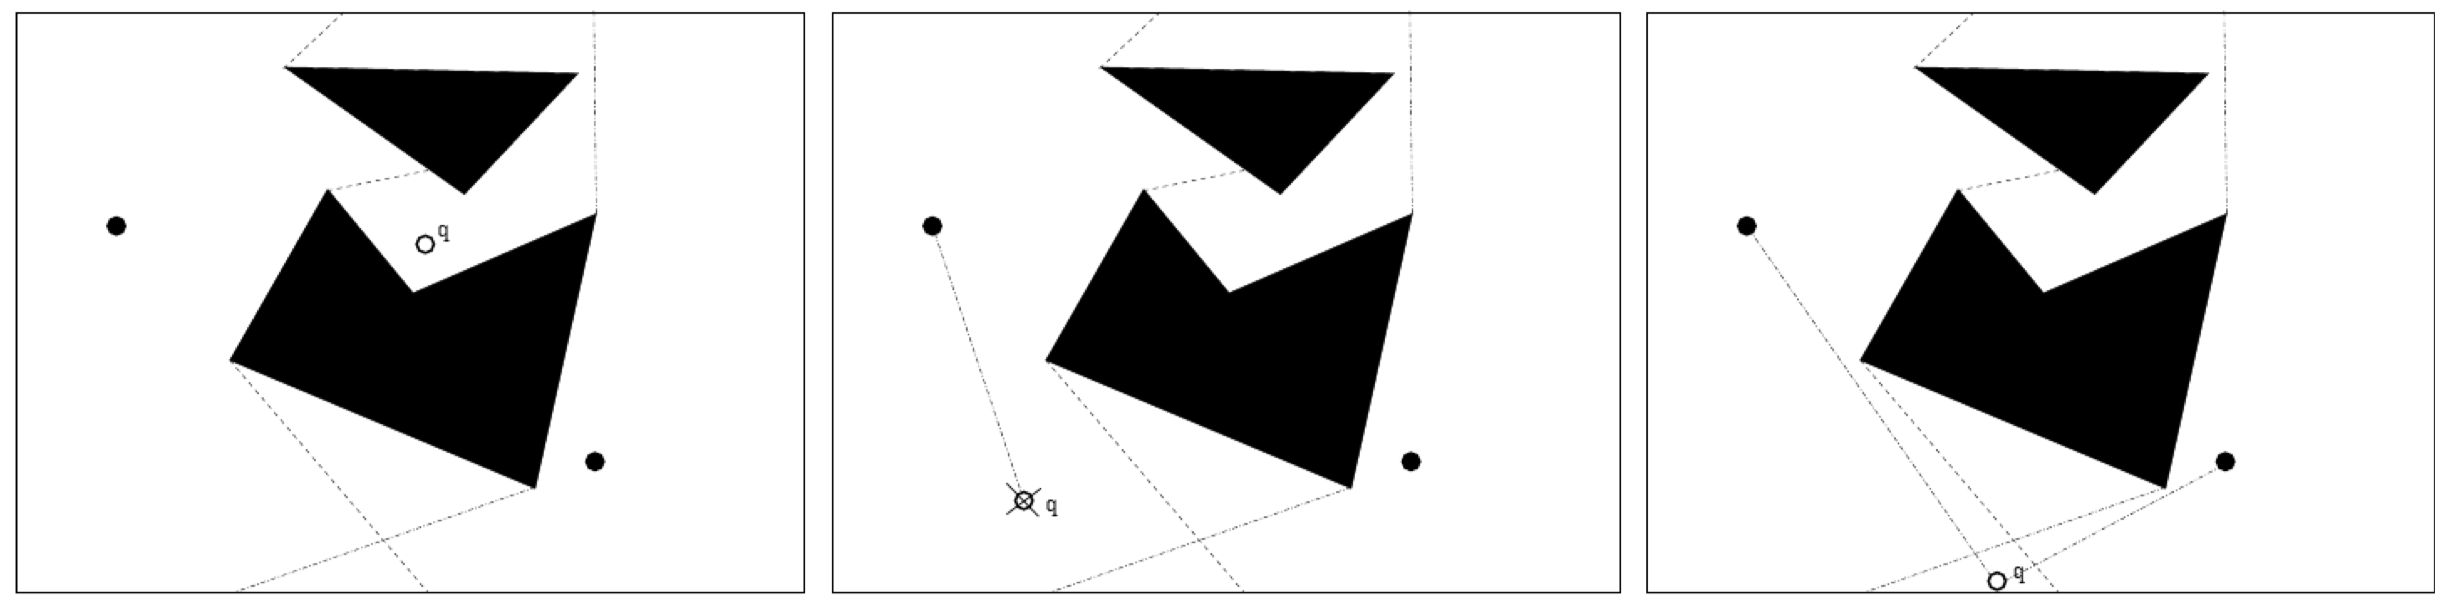
\includegraphics[width=15cm]{visibility_prm_visual}
\centering
\caption{node added as a guard; node rejected; connection node merging two connected components}
\label{fig:visprm_visual}
\end{figure}

\subsubsection{Principle}
The algorithm that we propose below is general. It allows us to build visibility
roadmaps without requiring any explicit computation of the visibility domains.
The roadmap is constructed incrementally by randomly sampling the configuration
space and attempting to connect some pairs of collision-free samples by the
local method. Figure \ref{fig:visprm_visual} illustrates the principle of the sampling strategy used at
each iteration of the algorithm. Randomly chosen configurations are checked for
collision to generate samples in $C_{free}$; when a free sample is found, it is added to
the roadmap either if it does not ‘see’ any another node of the current roadmap (i.e.
it is a new guard) or if it is seen by at least two nodes belonging to two distinct
connected components of the roadmap (i.e. it is a connection node). The end of
the roadmap’s construction is controlled by a termination condition related to the
volume of free space currently covered by the roadmap.

\subsubsection{Guard and connection node}
When a free sample is found, it is added to the roadmap in two cases:
\begin{itemize}
\item If it does not “see” another node already in R . This will be a new guard.
\item If it is seen at least by two nodes belonging to two distinct connected components of will be a connection node.
\end{itemize}
\subsubsection{Algorithm}

\begin{algorithm} 
\caption{Visibility\_PRM\_Algorithm} 
\label{alg:prm_alg} 
  \begin{algorithmic}[1]

    \STATE $Guard \leftarrow \emptyset$ 
    \STATE $Connection \leftarrow \emptyset$
    \STATE $ntry \leftarrow 0$
    \WHILE {$ntry < n$}
    \STATE $q \leftarrow$ a random configuration in $Q$     
    \STATE $g_{vis} \leftarrow \emptyset$
    \STATE $G_{vis} \leftarrow \emptyset$
    \FORALL {Conponents $G_{i}$ of $Guard$}
        \REPEAT
        \STATE $found \leftarrow FALSE$
          \FORALL {$nodes g \in g_{i}$}
              \IF {$q$ belongs to $Vis(g)$} 
                \STATE $found \leftarrow TRUE$
              \ENDIF
              \IF {$g_{vis} = \emptyset$}
                  \STATE $g_{vis} \leftarrow g$
                  \STATE $G_{vis} \leftarrow G_{i}$
              \ENDIF
              \ELSE
                  \STATE Add $q$ to Connection;
                  \STATE Create edges ($q$, $g$) and ($q$,$g_{vis}$)
                  \STATE Merge components $G_{vis}$ and $G_{i}$
          \ENDFOR
          \UNTIL {$found$=$TRUE$}
          \IF {$g_{vis}$ = $\emptyset$}
              \STATE add{$q$} to $Guard$
              \STATE $ntry \leftarrow 0$
          \ENDIF
          \ELSE
              \STATE $ntry$ = $ntry+1$
      \ENDFOR
  \ENDWHILE
    \end{algorithmic}
\end{algorithm}


The algorithm, called Visib-PRM, iteratively processes two sets of nodes: Guard
and Connection. The nodes of Guard belonging to a same connected component
(i.e. connected by nodes of Connection) are gathered in subsets $G_i$.


At each elementary iteration, the algorithm randomly selects a collision-free
configuration q. The main loop processes all the current components $G_i$ of Guard. The algorithm loops over the nodes g in $G_i$ , until it finds a node visible from q. The
first time the algorithm succeeds in finding such a visible node g, it memorizes both
g and its component $G_i$, and switches to the next component $G_{i+1}$. When q ‘sees’
another guard g$'$ in another component $G_j$ , the algorithm adds q to the Connection
set and the component $G_j$ is merged with the memorized $G_i$. If q is not visible from
any component, it is added to the Guard set. The main loop fails to create a new
node when q is visible from only one component; in that case q is rejected.\\
Parameter \textit{ntry} is the number of failures before the insertion of a new guard node.
1/\textit{ntry} gives an estimation of the volume not yet covered by visibility domains.
It estimates the fraction between the non-covered volume and the total volume of
$C_{free}$. This is a critical parameter which controls the end of the algorithm. Hence,
the algorithm stops when \textit{ntry} becomes greater than a user set value M, which
means that the volume of the free space covered by visibility domains becomes
probably greater than (1-1/M).
\subsubsection{Failure}
\begin{figure}[h]
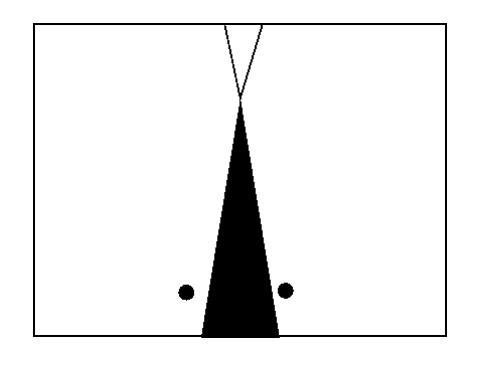
\includegraphics{visibility_prm_failure}
\centering
\caption{Visibility PRM Failure}
\label{fig:visprm_failure}
\end{figure}
The random generation of the guards may produce in some cases guards that will
be difficult to connect. This effect is illustrated in Fig. \ref{fig:visprm_failure} where two guards have
been generated near the boundary of the black triangular obstacle. They fully cover
$C_{free}$, however the intersection of both visibility domains is ‘unfortunately’ small.
The only way to complete the roadmap is to pick a connection node in the small
triangle. Then the algorithm will fail if the parameter M is not sufficiently high. Nevertheless this case is only a side-effect of the algorithm. Indeed, in this example,
the probability to select the first two guards with a small intersection domain is very
low. Moreover, this undesirable effect was never observed in practice in all the
examples we experimented on with the algorithm.

\end{document}
